% !TEX root = ./main.tex
% !TEX encoding = UTF-8 Unicode
% !TEX program = pdflatex
% !TeX spellcheck = it_IT

\chapter{Influence Maximization}
In questo capitolo verrà mostrata la creazione del grafo relativo alla \textit{Social Network}
e l'algoritmo di \textit{Influence Maximization} applicato su di esso.

\section{Creazione del grafo}
Nel precedente capitolo è stata illustrata la caratterizzazione dei nodi (lo score
assegnato ad ogni utente) e la creazione delle relazioni tra essi, con il relativo
peso associato.\\
Per la creazione del grafo è stato utilizzato il framework \textit{\textbf{Graphx}},
il quale permette di definire un oggetto di tipo grafo a partire da un \textit{VertexRDD},
contenente i nodi, e un \textit{EdgeRDD} contenente le relazioni con i relativi pesi.\\
Di seguito è riportato il codice.

\begin{figure}[!htbp]
	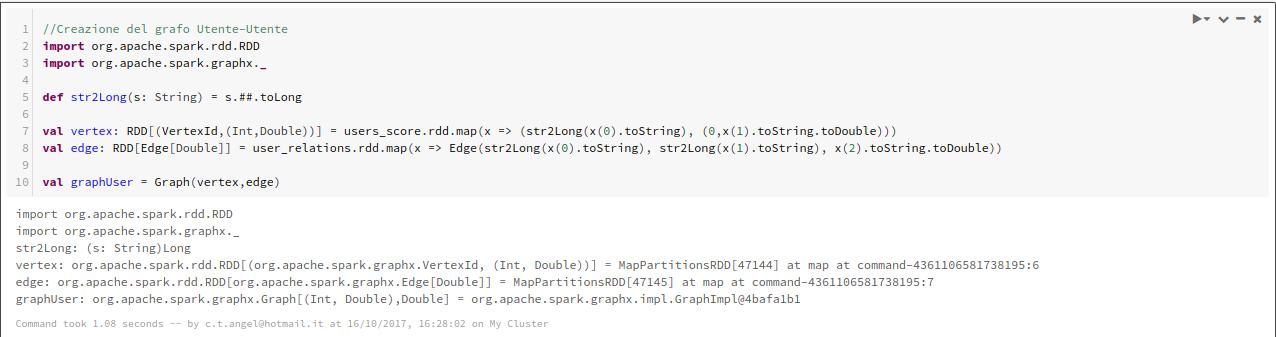
\includegraphics[width=1\linewidth,keepaspectratio]{command_17}
	\caption{Creazione del grafo}
	\label{command_17}
\end{figure}
\clearpage

\section{Algoritmo di Influence Maximization}
L'idea di base dell'algoritmo di Influence Maximization è la seguente: dato il
grafo delle rete sociale ottenuto, avente uno score per ogni nodo ed un peso per
ogni arco, individuare un numero finito di nodi da cui iniziare la copertura del
grafo e propagare l'influence, se e solo se, tale valore supera una soglia prefissata.\\
Per mostrare l'algoritmo utilizzato si consideri il grafo d'esempio in figura.

\begin{figure}[!htbp]
  \begin{center}
    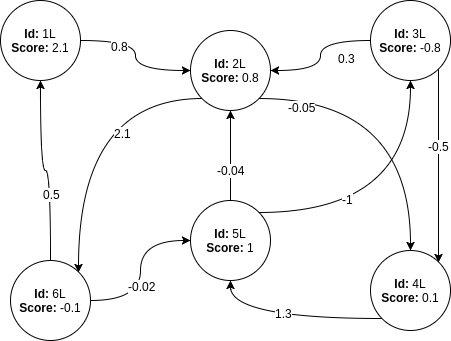
\includegraphics[width=0.6\linewidth,keepaspectratio]{step0}
  	\caption{Grafo d'esempio}
  	\label{step0}
  \end{center}
\end{figure}

\clearpage

Adesso, a fini illustrativi, si considera come nodo di partenza quello avente
score maggiore(evidenziato in verde).\\
Successivamente, invece, verrà illustrata la tecnica utilizzata nell'algortimo di \textit{spread}
per selezionare i nodi di partenza.\\
Nelle figure a seguire, tutti i nodi influenzati saranno evidenziati in verde.
\begin{figure}[!htbp]
  \begin{center}
    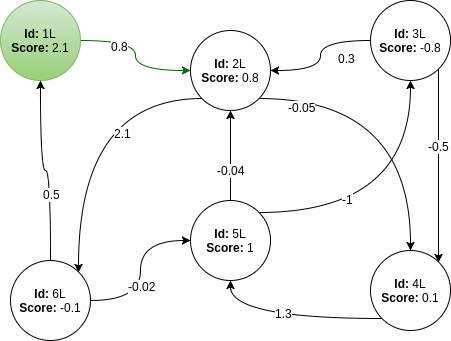
\includegraphics[width=0.6\linewidth,keepaspectratio]{step1}
  	\caption{Scelta nodo di partenza}
  	\label{step1}
  \end{center}
\end{figure}
\clearpage
Ciò che adesso viene illustrato, è il meccanismo di diffusione dell'influenza nel
grafo.//
Il nodo di partenza ha un solo arco in uscita, quindi invierà un messaggio contenete il proprio valore e
la media tra il proprio score ed il peso associato all'arco.\\
Il messaggio ha la seguente struttura $(score\_src, 0.5*score\_src+0.5*weight\_edge)$.\\
Una volta ricevuto il messaggio, il nodo destinazione controlla se il secondo valore è maggiore di una certa soglia,
ad esempio 0.\\
Qualora il confronto risulti positivo il nodo viene marcato come influenzato ed il
suo score sarà aggiornato con il minimo tra lo score sorgente(moltiplicato per un costante 0.5) ed il proprio score.\\
In \figurename~\ref{step2} è riportato il primo step: in particolare si noti che il nodo
risulta essere influenzato, ma il suo score non varia essendo il minimo tra 2.1*0.5 e 0.8.

\begin{figure}[!htbp]
  \begin{center}
    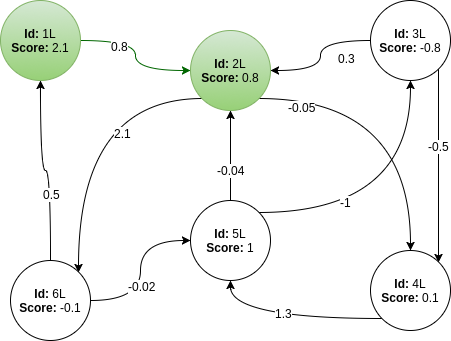
\includegraphics[width=0.6\linewidth,keepaspectratio]{step2}
  	\caption{Passo uno}
  	\label{step2}
  \end{center}
\end{figure}
\clearpage
L'algoritmo continua fintantoché tutti i nodi sono influenzati oppure non esistono più cammini percorribili.\\
Quindi tornando all'esempio, nel secondo step saranno influenzati i nodi \textbf{6L} e \textbf{4L}.

\begin{figure}[!htbp]
  \begin{center}
    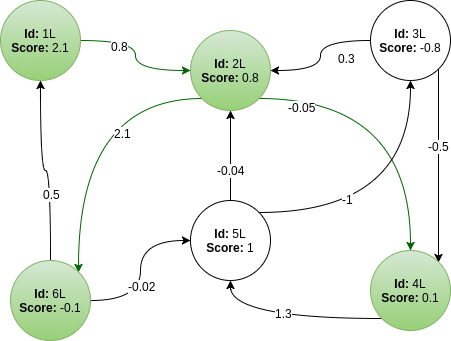
\includegraphics[width=0.6\linewidth,keepaspectratio]{step3}
  	\caption{Passo due}
  	\label{step3}
  \end{center}
\end{figure}
\clearpage
Nel terzo step si noti che il nodo \textbf{5L} ha due archi in ingesso, sui quali riceve simultaneamente
due messaggi.\\
In tal caso è considerato valido il messaggio avente arco con peso maggiore.
Lo score del nodo è aggiornato, essendo maggiore del valore ricevuto nel messaggio.\\
\begin{figure}[!htbp]
  \begin{center}
    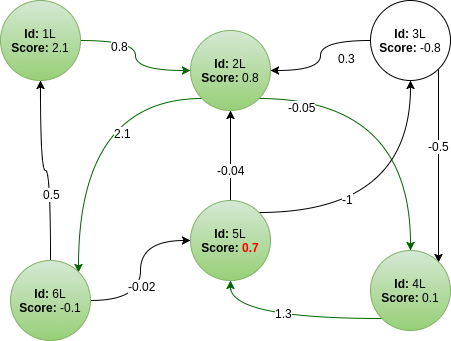
\includegraphics[width=0.6\linewidth,keepaspectratio]{step4}
  	\caption{Passo tre}
  	\label{step4}
  \end{center}
\end{figure}
\clearpage

Nel ultimo step, si noti che il nodo \textbf{3L}, marcato di rosso, non è stato influenzato
in quanto il valore non supera la soglia.
\begin{figure}[!htbp]
  \begin{center}
    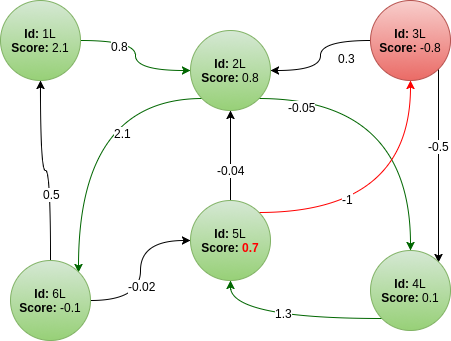
\includegraphics[width=0.6\linewidth,keepaspectratio]{step5}
  	\caption{Passo quattro}
  	\label{step5}
  \end{center}
\end{figure}
\clearpage
\subsection{Scelta utenti di partenza}
In questo paragrafo sarà discusso il criterio con cui sono stati scelti gli utenti
dai quali l'algoritmo di IM inizierà. In teoria di potrebbero tentare tutte le
possibili combinazioni, ma ciò richiederebbe un tempo computazionale elevato.\\
L'idea di base è quella di prendere un numero finito di combinazioni dove in ogni
combinazione i nodi non siano vicini tra loro. \\
Dato che la il grafo che stiamo esaminando, essendo una social network,
presenta dei cluster l'idea è quella di utilizzare un'algoritmo
di clustering per poi scegliere i nodi nei cluster più fitti, e in particolare scegliere gli
N nodi con score maggiore. Per i limiti hardware imposti da Databricks si è pensato di
scegliere un massimo di 5 cluster e 2 nodi in ogni cluster, così facendo andremo a testare
32 combinazioni differenti.\\
L'algoritmo di clustering scelto è Markov Cluster(MCL), tale algoritmo è basato sulle
catene di Markov. Per individuare un cluster in un grafo, MCL utilizza una matrice stocastica
e il concetto di random walks. In pratica le random walks tra due nodi sono più frequenti se esse appartengono
allo stesso gruppo. Così facendo si calcola la probabilità che un nodo ricade in
un cluster o in un altro.\\
L'algoritmo è diviso in tre fasi, le prime due simulano le random walks mentre la terza effettua una test di
convergenza. Nel dettaglio
\begin{itemize}
  \item \textbf{Expansion}: calcola il quadrato della Matrice Stocastica;
	\item \textbf{Inflation}: applica il prodotto di Hadamard sulla matrice sto
\end{itemize}
Di seguito è riportato il codice in cui è utilizzato tale algoritmo.
\begin{figure}[!htbp]
  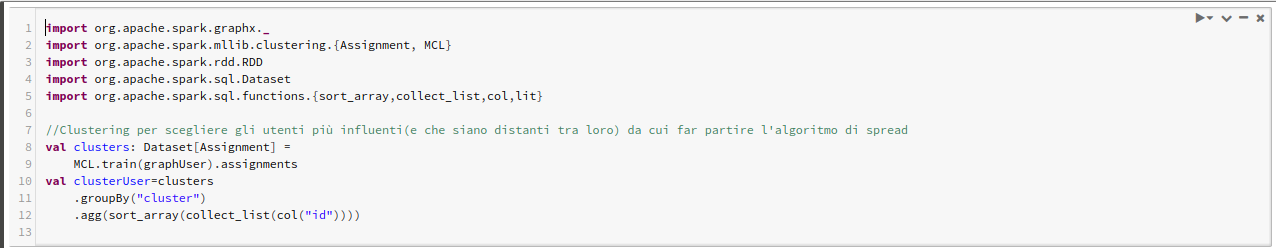
\includegraphics[width=1\linewidth,keepaspectratio]{command_18}
  \caption{Clustering}
  \label{command_18}
\end{figure}
\clearpage
Data che l'algoritmo di clustering utilizzato non conto dei valori presenti nei
nodi si sono dovuti recuperare il valore dello score, inoltre si sono estratti gli
id dei cluster con più di 250 nodi, infine si sono ottenuti 2 nodi per ogni cluster
dove i due nodi sono quelli con score maggiore nel proprio cluster, di seguito è riportato il codice.
\begin{figure}[!htbp]
  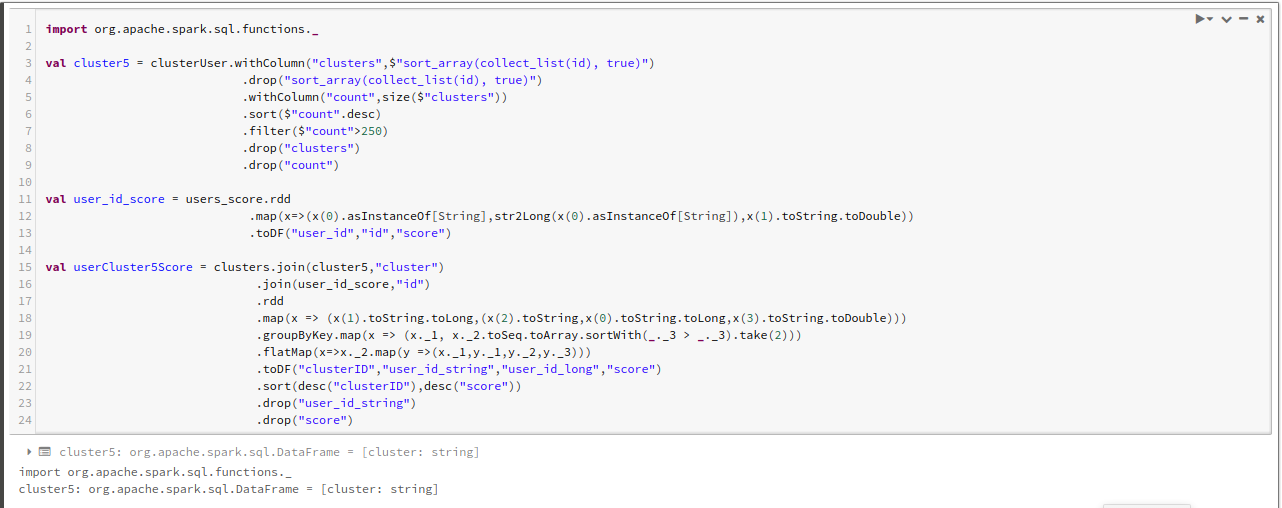
\includegraphics[width=1\linewidth,keepaspectratio]{command_20}
  \caption{Nodi di partenza}
  \label{command_20}
\end{figure}
Nella seguente figura è riportato il codice per l'estrazione delle combinazioni di
nodi da utilizzare come nodi di start.
\begin{figure}[!htbp]
  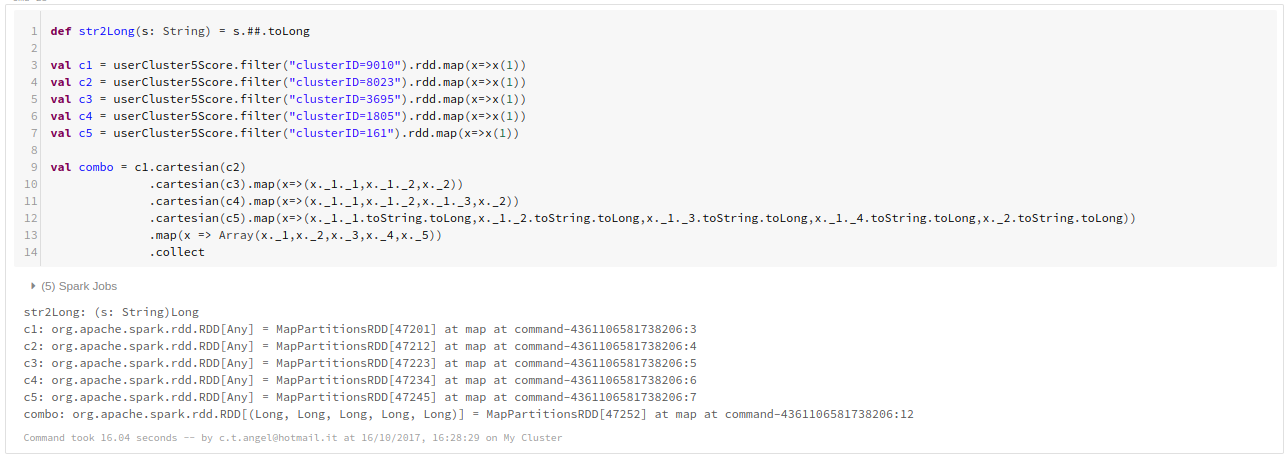
\includegraphics[width=1\linewidth,keepaspectratio]{command_23}
  \caption{Nodi di partenza}
  \label{command_23}
\end{figure}
\clearpage

\subsection{Scelta della soglia}
La soglia per cui si decide se un nodo è influenzato o meno dal precedente è stato
calcolata come media della mediana degli score degli utenti e della mediana dei pesi
degli archi, di seguito il codice.

\begin{figure}[!htbp]
  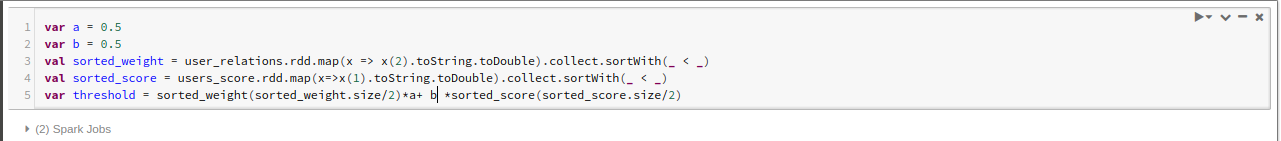
\includegraphics[width=1\linewidth,keepaspectratio]{command_24}
  \caption{Nodi di partenza}
  \label{command_24}
\end{figure}
\clearpage

\subsection{Implementazione in scala}
Per l'implementazione dell'algoritmo in Scala si è fatto uso della funzione \textit{\textbf{Pregel}}
messa a disposizione da \textit{\textbf{Graphx}}.\\
Pregel implementa uno scambio di messaggi tra nodi, tale funzione permette di definire tre
metodi:
\begin{itemize}
	\item \textbf{MergeMsg}: nel caso in cui il nodo riceve messaggi da più sorgenti permette
	di scegliere il criterio con cui scegliere il messaggio;
	\item \textbf{vProg}: permette di effettuare delle operazioni nel nodo.
	\item \textbf{SendMsg}: permette di definire in che modo un nodo deve inviare i messaggi.
\end{itemize}
L'esecuzione di \textit{\textbf{Pregel}} è suddivisa in super step e in ogni uno di essi
sono eseguiti metodi sopra descritti.\\
Inoltre si possono specificare altri parametri come: numero massimo di iterazioni e messaggio iniziale.\\
Nella figura è riportato il codice per la definizione delle funzioni: \textbf{MergeMsg}, \textbf{vPorg} e \textbf{SendMsg}.
\begin{figure}[!htbp]
  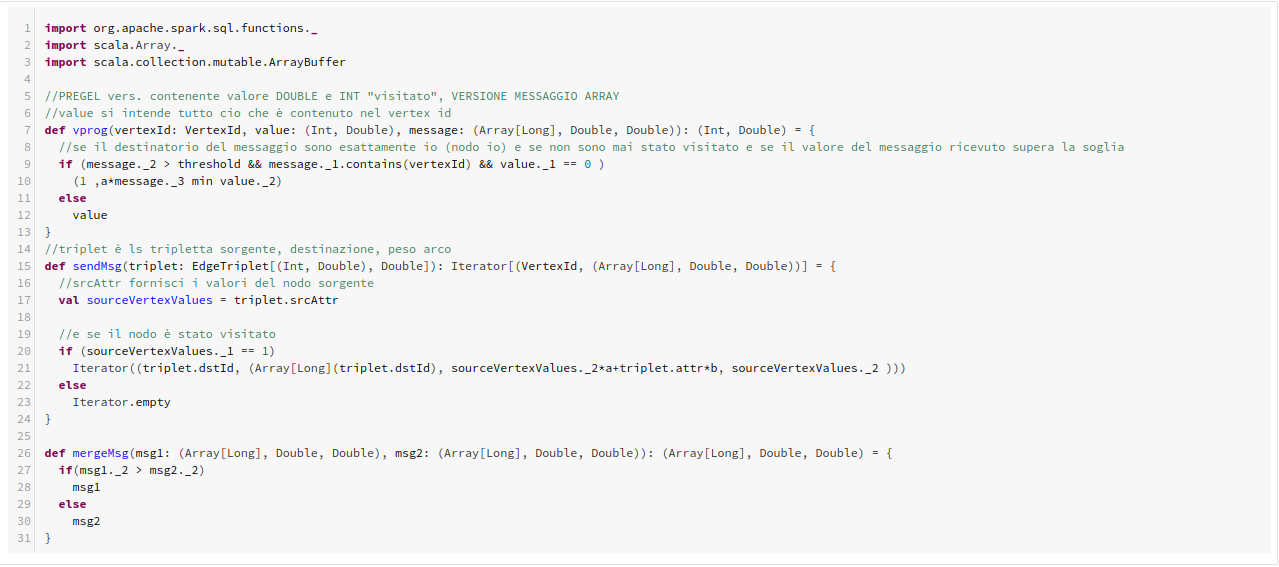
\includegraphics[width=1\linewidth,keepaspectratio]{command_25}
  \caption{Definizione MergeMsg, vProg, SendMsg}
  \label{command_25}
\end{figure}
\clearpage

Nella seguente figure è riportato il codice la l'esecuzione dell'algoritmo per ogni combinazione è l'estrazione
del risultato con maggiore copertura.
\begin{figure}[!htbp]
  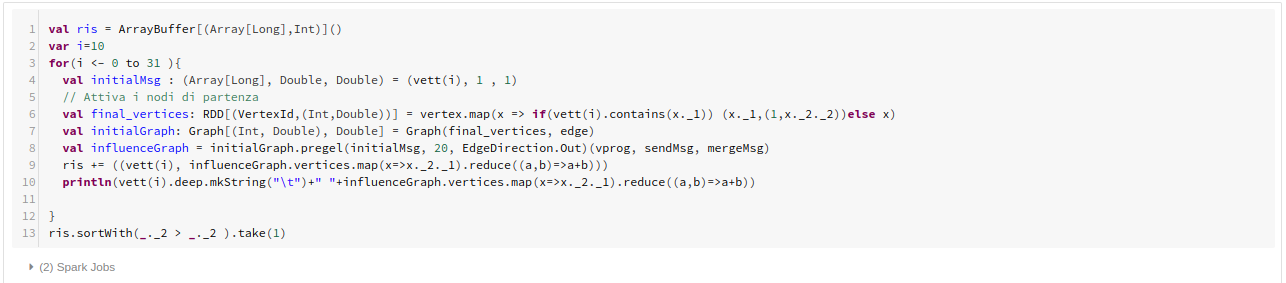
\includegraphics[width=1\linewidth,keepaspectratio]{command_26}
  \caption{Esecuzione Pregel}
  \label{command_26}
\end{figure}
\clearpage
